\chapter{Gelijkstroommachines (DC Machines)}
DC-machines zijn dus elektrische machines die werken op een gelijkspanning, ze zijn
makkelijk te regelen (vooral vroeger was dit zo, nu zijn andere motoren ook makkelijker
regelbaar dus wordt deze machine minder gebruikt).
Ze kunnen klein zijn en ook groot zijn, klein omdat ze permanente magneten gebruiken en
zeldzame elementen (vaak niet zo duurzaam wel), het gewicht kan soms belangrijk zijn, wat
die permanente magneten dus voordelig maakt.

\section{Werkingsprincipe}
Er zijn verschillende principes die zorgen voor de werking van de DC-machine, dit zijn de
\textbf{wet van Faraday-Lenz}, \textbf{wet van Lorentz} en de \textbf{wet van Ampère}.

\subsection{Wet van Ampère}
Deze wet heeft niet direct veel invloed op de werking van de DC-machine (als je permanente
magneten hebt!) maar is wel belangrijk om te weten.
Deze wet beschrijft de relatie tussen een elektrische stroom en het magnetisch veld dat
deze stroom opwekt.
De wet van Ampère kan worden uitgedrukt met de volgende formule:
\begin{align*}
    \oint_l \vv{B} \cdot d\vv{l} = \mu_0 \cdot i
\end{align*}
Met de \textit{rechterhand regel} kan de richting van het magnetisch veld bepaald worden.
Indien je geen permanente magneten gebruikt, gebruik je wikkelingen in de stator, het is
juist deze wet dat dan eigelijk gebruikt wordt om het veld op te wekken en te bepalen hoe
hard dat veld is.
Moest je permanente magneten hebben is er inderdaad niet veel invloed op de werking maar
gaat er wel nog steeds wat invloed zijn op het veld want de rotor heeft ook stroomvoerende
geleiders, het totaal veld gaat een beetje vervormen (Ankerreactie) maar dit zien we
later.

\begin{figure}[H]
  \centering
  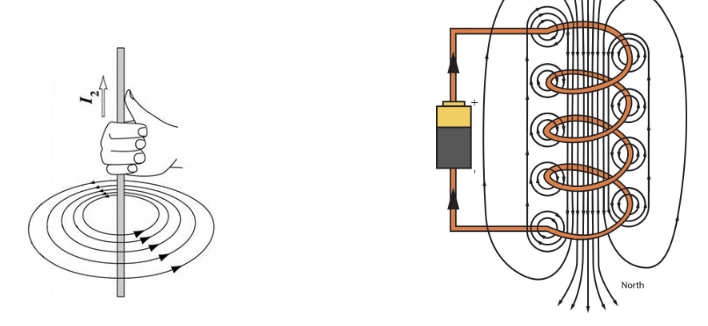
\includegraphics[width=0.6\textwidth]{assets/wetampere.png}
  \caption{Wet van Ampère}
  \label{fig:wetampere.png}
 \end{figure}

Dit kan ook zorgen voor wat lekflux, maar dit zien we later.

\subsection{Wet van Lorentz}
Vooraleer we naar het effectieve werkingsprincipe gaan kijken van de DC-motor, gaan we
eerst kijken naar de wet van Lorentz.
Deze wet beschrijft de kracht die een geladen deeltje ondervindt wanneer het zich in een
magnetisch veld bevindt.
De kracht wordt gegeven door de formule:
\begin{align*}
    \vv{F} = q \cdot \vv{E} + q \cdot \vv{v} \times \vv{B}
\end{align*}
Hierbij is $\vv{F}$ de kracht op het deeltje, $q$ de lading van het deeltje, $\vv{E}$ het
elektrische veld, $\vv{v}$ de snelheid van het deeltje en $\vv{B}$ het magnetisch veld.
Dit is niet echt belangrijk om te kennen maar wat wel belangrijk te weten is dat deze
formule herschreven kan worden voor een stroomvoerende geleider in een magnetisch veld
(een toepassing op de wet van Lorentz).:
\begin{align*}
    \vv{F} = I \cdot \vv{L} \times \vv{B}
\end{align*}
Hierbij is $I$ de stroom door de geleider, $\vv{L}$ de lengte van de geleider in het
magnetisch veld en $\vv{B}$ het magnetisch veld.
De kracht is dus loodrecht op zowel de stroomrichting als het magnetisch veld, dit is
essentieel voor de werking van de motor, want hierdoor ontstaat er een koppel dat de rotor
doet draaien.
Met de \textit{Linkerhand regel} kan je de richting bepalen:

\begin{figure}[H]
  \centering
  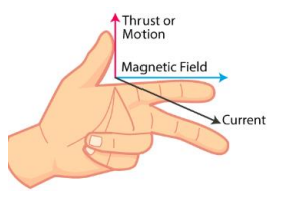
\includegraphics[width=0.3\textwidth]{assets/linkerhandregel.png}
  \caption{Linkerhandregel}
  \label{fig:linkerhandregel.png}
 \end{figure}

Als we nu zo een stroomvoerende geleider in een lus in een magnetisch veld plaatsen, zal
er een moment ontstaan dat de lus doet draaien.
Dit is het basisprincipe van de DC-motor.
De richting van de stroom en het magnetisch veld bepalen de draairichting van de motor.
De volledige bewerking van het uiteindelijk resultaat van dat moment ga ik hier niet
uitrekenen maar op de slide staat dan dat het moment uitendelijk als volgt beschreven
wordt:
\begin{align*}
    M = N \cdot i \cdot S \cdot B \cdot sin(\theta)
\end{align*}
Hierbij is $M$ het koppel, $N$ het aantal windingen in de lus, $S$ het oppervlak van de
lus, $i$ de stroom door de lus, $B$ de magnetische fluxdichtheid en $\theta$ de hoek
tussen het oppervlak van de lus en het magnetisch veld.

\begin{figure}[H]
  \centering
  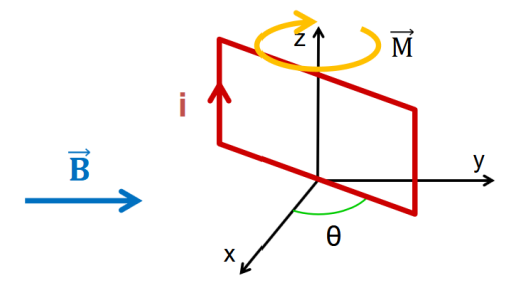
\includegraphics[width=0.4\textwidth]{assets/strromlus.png}
  \caption{Stroomlus in een magnetisch veld}
  \label{fig:strromlus.png}
 \end{figure}

\newpage

\subsection{Wet van Faraday-Lenz}
De laatste wet die we nodig hebben is die van Faraday-Lenz.
Deze beschrijft dat er een spanning (EMK) wordt opgewekt wanneer een geleider door een
magnetisch veld beweegt, en dat die opgewekte spanning zich volgens Lenz net zo richt dat
ze de oorzaak tegenwerkt.
Voor een geleider die met een snelheid $v$ door een veld $B$ beweegt, geldt:
\begin{align*}
    e = B \cdot l \cdot v
\end{align*}
Hierbij is $e$ de opgewekte spanning (EMK), $B$ de magnetische fluxdichtheid, $l$ de
lengte van de geleider in het veld en $v$ de snelheid waarmee de geleider beweegt.
(Dit komt eigelijk van $\vv{E} = \vv{v} \times \vv{B}$, en de vorm $e = B \cdot l \cdot v$
klopt alleen als alles loodrecht is.)

In de DC-motor speelt dit een belangrijke rol.
Zodra de rotor draait, bewegen zijn geleiders door het magnetisch veld, en volgens de
formule hierboven wekken ze dus zelf een spanning op.
Volgens Lenz is die tegengesteld aan de aangelegde voedingsspanning, en daarom noemen we
ze de \textbf{tegen-EMK} (of back-EMF).
Hoe sneller de rotor draait (grotere $v$), hoe groter deze tegen-EMK.

De aangelegde spanning $U$ moet dus in evenwicht zijn met deze tegen-EMK $E$ plus de
spanningsval over de ankerweerstand $R$:
\begin{align*}
    U = E + I \cdot R
\end{align*}
Hieruit volgt meteen het gedrag van de motor.
Bij het opstarten staat de rotor stil, dus $v = 0$ en $E = 0$, waardoor de aanloopstroom
$I = U/R$ heel groot is.
Naarmate de motor op snelheid komt, stijgt $E$, wordt $(U - E)$ kleiner en daalt de stroom
vanzelf.
De motor regelt zichzelf dus:
hij trekt net genoeg stroom voor de belasting die op de as staat.

Ten slotte toont deze wet ook de \textbf{dualiteit motor--generator}.
Dezelfde machine kan in twee richtingen werken.
Als motor stop je er elektrische energie in en komt er mechanische energie (koppel) uit,
waarbij de tegen-EMK een neveneffect is dat de stroom begrenst.
Draai je de as daarentegen mechanisch aan, dan beweegt de geleider door het veld en wekt
de machine via $e = B l v$ zelf een spanning op die je kunt afnemen:
ze werkt dan als \textbf{generator}.
De tegen-EMK in een draaiende motor is eigenlijk het bewijs dat die generatorwerking er
altijd al in zit; enkel de energierichting keert om.

\begin{figure}[H]
  \centering
  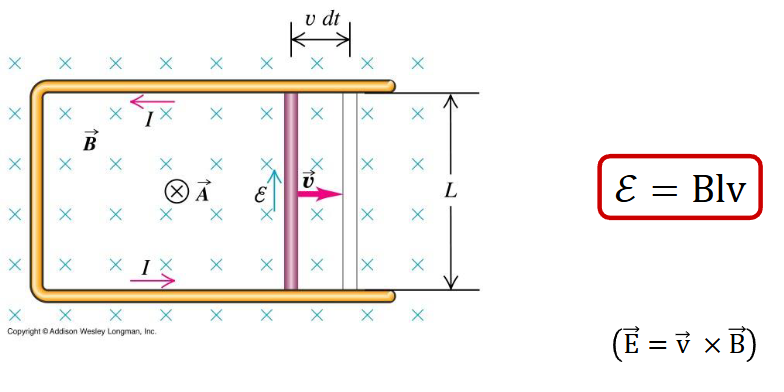
\includegraphics[width=0.6\textwidth]{assets/wetfaradaylenz.png}
  \caption{Werkingsprincipe Faraday-Lenz}
  \label{fig:wetfaradaylenz.png}
 \end{figure}

\subsection{Werkingsprincipe DC-motor}
Met deze wetten kan dus nu de werkingsprincipe van de DC-motor volledig verklaard worden,
ook duidelijk in de volgende figuur:

\begin{figure}[H]
  \centering
  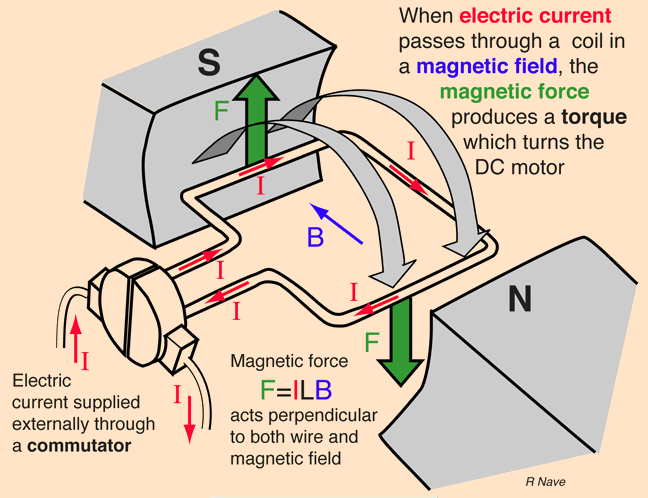
\includegraphics[width=0.5\textwidth]{assets/Faradaylenz.png}
  \caption{Werkingsprincipe DC-motor}
  \label{fig:Faradaylenz.png}
 \end{figure}

We zien hier dus een stroomvoerende lus in een magnetisch veld, de wet van Lorentz zegt
dat er dan een resulterende kracht is, die dus een moment genereert dat de motor doet
draaien.
De stroom wordt daar aangelegd met een \textbf{commutator} deze zorgt ervoor dat de
stroomrichting in de lus altijd zo is dat het moment in dezelfde richting blijft, dus de
stroomrichting in de lus wordt steeds omgekeerd als de lus een halve rotatie heeft
gemaakt.
Ook is er lekflux door de wet van Ampère en hebben we dus ook een tegen-emk.

\begin{figure}[H]
  \centering
  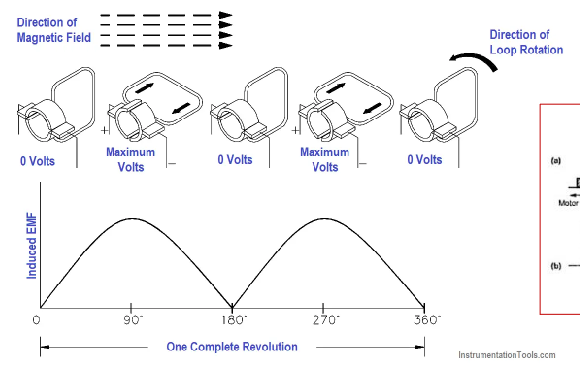
\includegraphics[width=0.6\textwidth]{assets/commutatorenemk.png}
  \caption{Commutator en geïnduceerd tegen-EMK in de DC-motor}
  \label{fig:commutatorenemk.png}
 \end{figure}

In de figuur hierboven zien we fysisch hoe die commutator werkt en ook het verloop van de
tegen-emk, je ziet dat de tegen-emk minimaal is daar waar de stroom door de lus net nul
is.
Dit is dus eigelijk ook voor 1 lus gerepresenteerd.
\textit{Een commutator is eigelijk een mechanische gelijkrichter.}

Voor meerdere wikkelingen, waar we dus sneller wisselen met commutatoren gaan we een
tegen-emk krijgen zoals op de volgende figuur:

\begin{figure}[H]
  \centering
  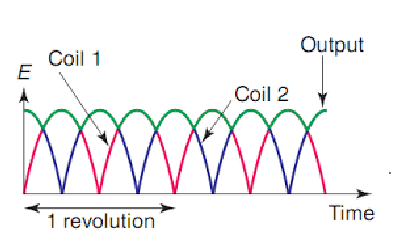
\includegraphics[width=0.6\textwidth]{assets/tegenemkmeerdere.png}
  \caption{Tegen-EMK in DC-motor met meerdere wikkelingen}
  \label{fig:tegenemkmeerdere.png}
 \end{figure}

Dit is dus een meer vlakkere curve, dit geldt dus ook voor het koppel:

\begin{figure}[H]
  \centering
  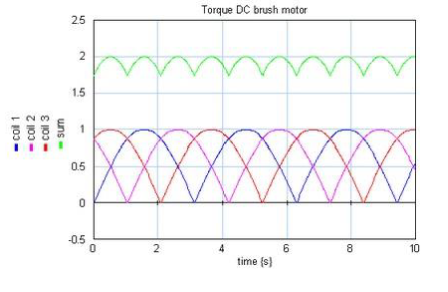
\includegraphics[width=0.6\textwidth]{assets/koppelmeerderelusse.png}
  \caption{Koppel in DC-motor met meerdere wikkelingen}
  \label{fig:koppelmeerderelusse.png}
 \end{figure}

Hier een close-up van de commutator, je ziet hier de koolstofborstels die er tegen duwen
zodat de stroom van de voeding naar de rotor kan gaan, je ziet ook een veer dat zorgt dat
de koolstofborstel goed tegen de commutator blijft duwen.

\begin{figure}[H]
  \centering
  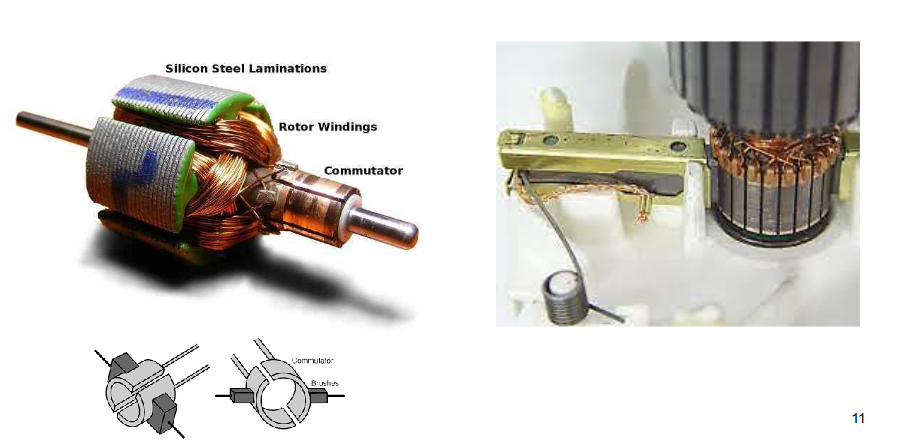
\includegraphics[width=0.6\textwidth]{assets/closeupcommutator.png}
  \caption{Close-up commutator}
  \label{fig:closeupcommutator.png}
 \end{figure}

\section{Constructie}
Dan gaan we nu eens de constructie van de DC-machine overlopen, we weten dus dat er een
stator en een rotor is, deze kunnen we ook zien in de volgende figuur:

\begin{figure}[H]
  \centering
  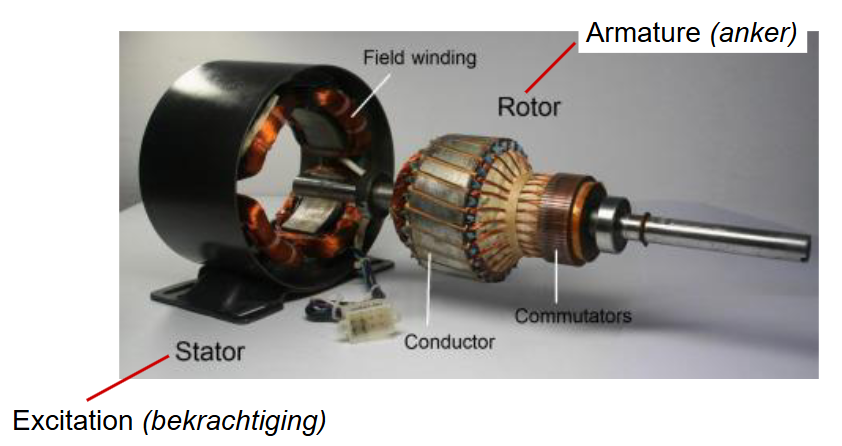
\includegraphics[width=0.6\textwidth]{assets/statorenrotordcmachine.png}
  \caption{Constructie van de DC-machine}
  \label{fig:statorenrotordcmachine.png}
 \end{figure}

De \textit{stator} staat bij de DC-machine \textit{vast} en bestaat meestal uit
geconcentreerde wikkelingen, bij de DC-machine wordt deze altijd de \textbf{excitatie},
\textbf{bekrachtiging} of het \textbf{veld} genoemd.
Die benaming komt van het feit dat je de wikkelingen in de stator een magnetisch veld doet
opwekken (als het dus met wikkelingen is).

\begin{figure}[H]
  \centering
  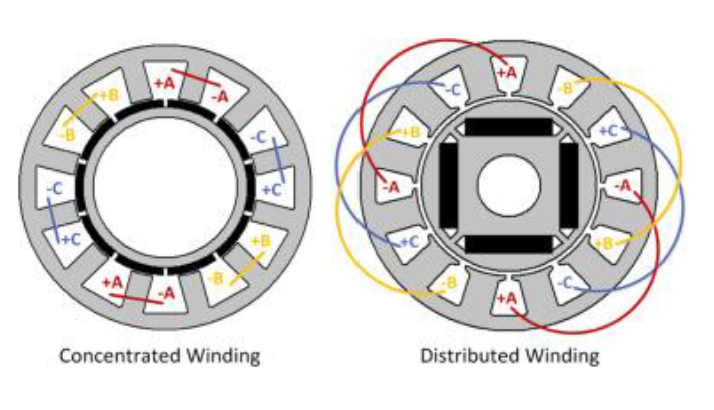
\includegraphics[width=0.6\textwidth]{assets/concrentregedstribitureed.png}
  \caption{Extra weergave van de statorconstructie met geconcentreerde en verdeelde
  wikkelingen}
  \label{fig:concrentregedstribitureed.png}
 \end{figure}

De \textit{rotor} is hier het draaiende deel van de machine, bij de DC-machine wordt deze
altijd het \textbf{anker} genoemd.
De rotor is bevestigd in de stator en draait rond een as.
We zien op de figuur hier ook nog de commutators (er zijn meerdere wikkelingen).

Nog een eigenschap van een DC-machine is het \textbf{poolpaartal} (hoeveel duos van
polen), die polen vormen het magnetisch veld (elk pool maakt een veld), maar je kan dus
meerdere poolpaartallen hebben, meer poolpaartallen zorgen er ook voor dat je de motor
trager kan laten draaien.
Elk poolpaar geeft namelijk één veldwisseling per omwenteling, dus met meer polen ziet de
rotor meer veldwisselingen per toer.
Zo maakt de machine nog genoeg spanning en koppel, zelfs als de as traag draait.
Met weinig polen zou je bij die lage snelheid te weinig veldwisselingen hebben en zou je
de motor juist snel moeten laten draaien.
Daarom vind je veel polen vooral bij grote, traag draaiende machines met veel koppel.

\newpage

Er zijn wel nadelen aan veel polen.
Elke pool neemt met zijn wikkeling plaats in op de omtrek, dus heb je een grotere diameter
nodig om ze kwijt te kunnen.
Ook keert het veld sneller om in de rotor, wat meer ijzerverliezen geeft.
Voor een gewone, snelle en compacte motor houd je het poolpaartal dus liefst laag, typisch
2 tot 8 polen max.

\begin{figure}[H]
  \centering
  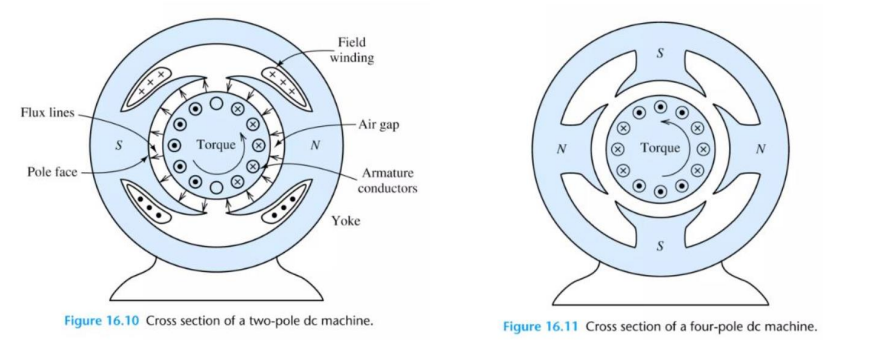
\includegraphics[width=0.6\textwidth]{assets/1en2poolpaartallendcmotor.png}
  \caption{DC-motor met 1 en 2 poolparen}
  \label{fig:1en2poolpaartallendcmotor.png}
 \end{figure}

Nog iets dat belangrijk is zijn de wikkelingen van de rotor, deze kunnen op verschillende
manieren verbonden zijn.
Het bepalen van hoe je ze verbindt hangt af van de gewenste nominale waarden voor
spanning, stroom, vermogen, enz.
Het wikkelen van de rotor kan er namelijk voor zorgen dat er minder stroom door elke
individuele geleider gaat.
Dit wordt duidelijker in de volgende figuur:

\begin{figure}[H]
  \centering
  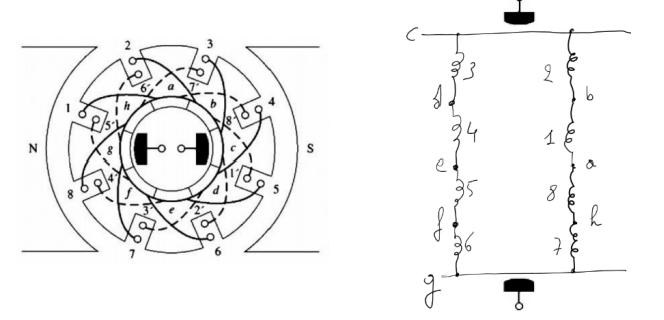
\includegraphics[width=0.8\textwidth]{assets/rotorwikkeling2poligiemotor.png}
  \caption{Rotorwikkeling van een 2-polige DC-motor}
  \label{fig:rotorwikkeling2poligiemotor.png}
 \end{figure}

Hierboven zien we een specifieke rotorwikkeling van een 2-polige DC-motor.
De 2 zwarte blokjes zijn eigenlijk de koolstofborstels op de commutator:
als het rechterblokje de + is, dan is het linkerblokje de -.
De verbinding gebeurt dan als volgt:
$+ \rightarrow 3 \rightarrow 3' \rightarrow 4 \rightarrow 4' \rightarrow 5 \rightarrow \cdots$.
We krijgen zo de schematische opstelling die we rechts zien:
2 parallelle takken, waardoor de stroom zich kan verdelen.

\section{Motor model en karakteristieken}
Om berekeningen in de praktijk vlotter te doen gaan we nu eens van ons meer fysisch model
dat we eerder hadden uitgelegd naar een mathematisch model gaan en effectief de formules
bezien.
Hiermee kunnen we dan uiteindelijk een equivalent schema opstellen en de karakteristieken
van de motor bepalen.

\subsection{Koppel}
We weten dat het koppel van de motor beschreven kan worden als:
\begin{align*}
    T = N \cdot F \cdot 2 \cdot r
\end{align*}
Hierbij is $T$ het koppel, $N$ het aantal windingen, $F$ de kracht op de geleider en $r$
de straal van de rotor.
Nu weten we dat de kracht op de geleider kan worden beschreven met de wet van Lorentz:
\begin{align*}
    T = N \cdot i_a \cdot l \cdot B \cdot 2 \cdot r
\end{align*}
Hierbij is $i_a$ de stroom door de ankerwikkeling, $l$ de 'actieve' lengte van de
rotorgeleider en $B$ de magnetische fluxdichtheid.
Met 'actieve' bedoelen we dus het deel van de geleider waar dus effectief een tegen-emk
wordt geïnduceerd.
Om dit te verduidelijken tekent de proff het volgende aan bord:

\begin{figure}[H]
  \centering
  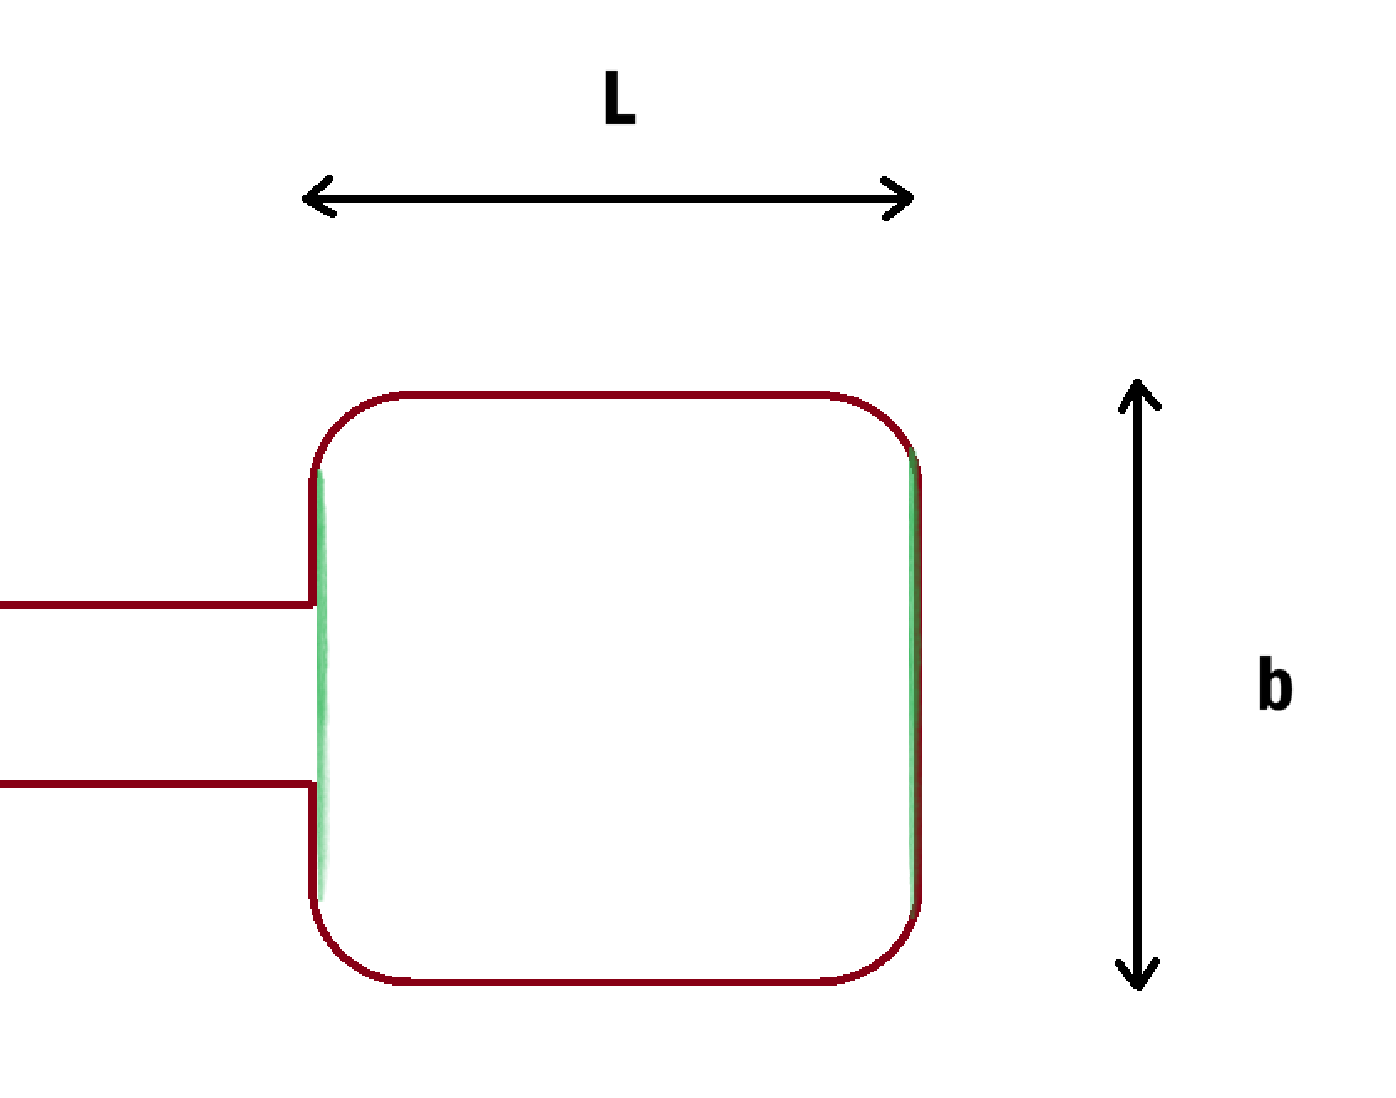
\includegraphics[width=0.4\textwidth]{assets/luswikkeling.png}
  \caption{1 wikkeling van de rotor}
  \label{fig:luswikkeling.png}
 \end{figure}

Het groen gearceerde heeft hier netto geen tegen-emk dat geïnduceerd wordt, het is dus
niet actief.
Het deel dat wel actief is, is het deel dat loodrecht staat op de veldlijnen van het
magnetisch veld.
Ook die $2r$ en l zijn samen eigelijk een oppervlakte en een oppervlakte vermenigvuldigd
met de magnetische inductie B is dus een flux, we kunnen dit dus herschrijven als:
\begin{align*}
    T = K \cdot \varphi \cdot i_a
\end{align*}
Hierbij is K een constante (soms wordt er ook C gebruikt)

Ook weten we dat deze flux $\varphi$ evenredig is met de veldstroom $i_f$ (of $i_e$) (de
stroom door de statorwikkelingen), dus we kunnen dit herschrijven als:
\begin{align*}
    T = G \cdot i_e \cdot i_a
\end{align*}

\newpage

\subsection{Tegen-EMK}
Met de wet van Faraday-Lenz kunnen we de tegen-EMK van de motor beschrijven als:
\begin{align*}
    E = B \cdot l \cdot v
\end{align*}
Alles moet wel loodrecht staan!
Bij een rotatie geldt ook dat de snelheid $v$ van de geleider kan worden beschreven als:
\begin{align*}
    v = \omega \cdot r
\end{align*}
Hierbij is $\omega$ de hoeksnelheid van de rotor en $r$ de straal van de rotor.
Ook weten we dat $l \cdot 2 \cdot r$ de oppervlakte van de lus is, en dat $B \cdot A$ de
flux door de lus is, dus we kunnen dit herschrijven als:
\begin{align*}
    E = K \cdot \varphi \cdot \omega
\end{align*}
Deze K is dezelfde constante als bij het koppel, dit is dus een constante die afhankelijk
is van de constructie van de motor.
Dit is 'interessant' bij DC-machines zegt de proff.

\subsection{Klemspanning}
Met de wetten van Kirchoff (KVL) kunnen we de klemspanning van de motor beschrijven als:
\begin{align*}
   U_a = E + R_a \cdot i_a + {\color{red}L_a \cdot \frac{di_a}{dt}}
\end{align*}
Hierbij is $U_a$ de klemspanning (van het anker dus), $E$ de tegen-emk die we eerder
beschreven hebben, $R_a$ de weerstand van de ankerwikkeling, $L_a$ de inductantie van de
ankerwikkeling en $i_a$ de stroom door de ankerwikkeling.
De term $L_a \cdot \frac{di_a}{dt}$ vertegenwoordigt de spanningsval over de inductantie
van de ankerwikkeling die geïnduceerd wordt, die optreedt wanneer de stroom door de
wikkeling verandert.
Deze is verwaarloosbaar bij een DC-machine omdat die zo klein is en dus niet bijdraagt aan
de klemspanning.
De effectieve formule die we gaan gebruiken voor de klemspanning is dus:
\begin{align*}
   U_a = E + R_a \cdot i_a
\end{align*}
Met deze 3 vergelijkingen kunnen we de hele DC-machine beschrijven, ook is het ideaal dat
deze allemaal lineair zijn.

\newpage

\subsection{Equivalent Schema}
Het opgestelde equivalent schema ziet er als volgt uit:

\begin{figure}[H]
  \centering
  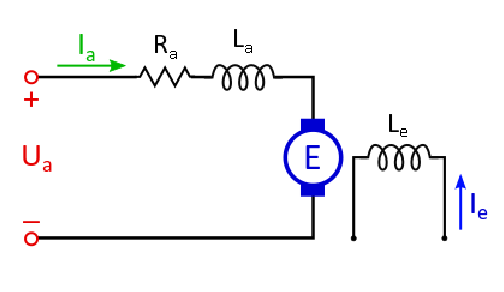
\includegraphics[width=0.6\textwidth]{assets/equivalentschemaDC.png}
  \caption{Equivalent schema van de DC-machine}
  \label{fig:equivalentschemaDC.png}
 \end{figure}

Het linkse gedeelte representeert het \textit{Rotormodel} en het rechtse gedeelte
representeert het \textit{Statormodel}.
Bij het statormodel is er eigelijk ook nog een weerstand in serie met $L_e$ ($R_e$) en wat
ook niet super duidelijk is, maar wel belangrijk te weten is dat die stator ook nog gevoed
wordt (veldvoeding), maar de manier waarop deze gevoed wordt kan verschillen (dit zien we
zometeen).
Bij dat rotormodel zijn die 2 blauwe blokjes bij E de weergave van de koolstofborstels.
De tegen-emk wordt eigelijk als spanningsbron gemodelleerd.

\subsection{DC-motor types}
Er zijn ook verschillende soorten motoren en \textit{bekrachtigingen} (hoe de stator wordt
gevoed, dus de excitatie).
De bekrachtiging kan op verschillende manieren gebeuren, dit zijn de volgende:

\begin{itemize}
  \item \textbf{Aparte excitatie}:
  Oftewel 'onafhankelijke bekrachtiging', hierbij wordt het anker en de excitatie door een
  andere bron gevoed, onafhankelijk van elkaar dus.
  Zelfde schema als eerder dus ook, alleen daar bij het statormodel gewoon een aparte
  voeding verbinden.
  \item \textbf{Shunt excitatie}:
  Hierbij plaatsen we de excitatie en het anker in parallel, dit heeft als voordeel een
  constante flux, dus het koppel is lineair met de ankerstroom, en de snelheid blijft vrij
  stabiel ongeacht van de belasting.
  Ideaal voor als je een constante snelheid wilt.
  \begin{figure}[H]
    \centering
    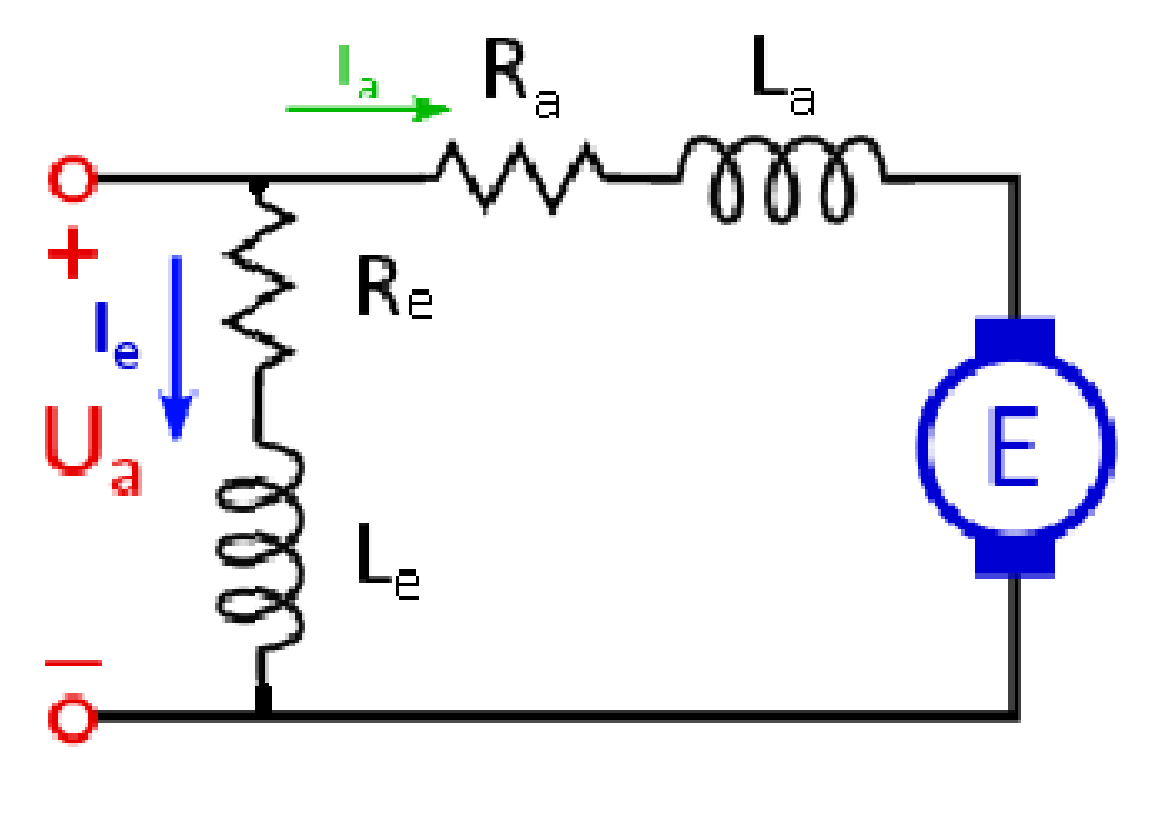
\includegraphics[width=0.5\textwidth]{assets/shuntbekrachtiging.png}
    \caption{Shunt bekrachtiging van een DC-machine}
    \label{fig:shuntbekrachtiging.png}
   \end{figure} 
   \newpage
   \item \textbf{Serie excitatie}:
   Hierbij plaatsen we de excitatie en het anker in serie, dit heeft als voordeel dat de
   excitatiestroom gelijk is aan de ankerstroom, waardoor met $T = G \cdot i_e \cdot i_a$
   het koppel kwadratisch stijgt met de stroom, waardoor er een groot startkoppel ontstaat
   bij lage snelheid/stilstand en dit koppel dan sterk daalt als de snelheid stijgt,
   perfect voor toepassingen die veel kracht nodig hebben om te starten maar daarna minder
   zoals een trein.
  \begin{figure}[H]
     \centering
     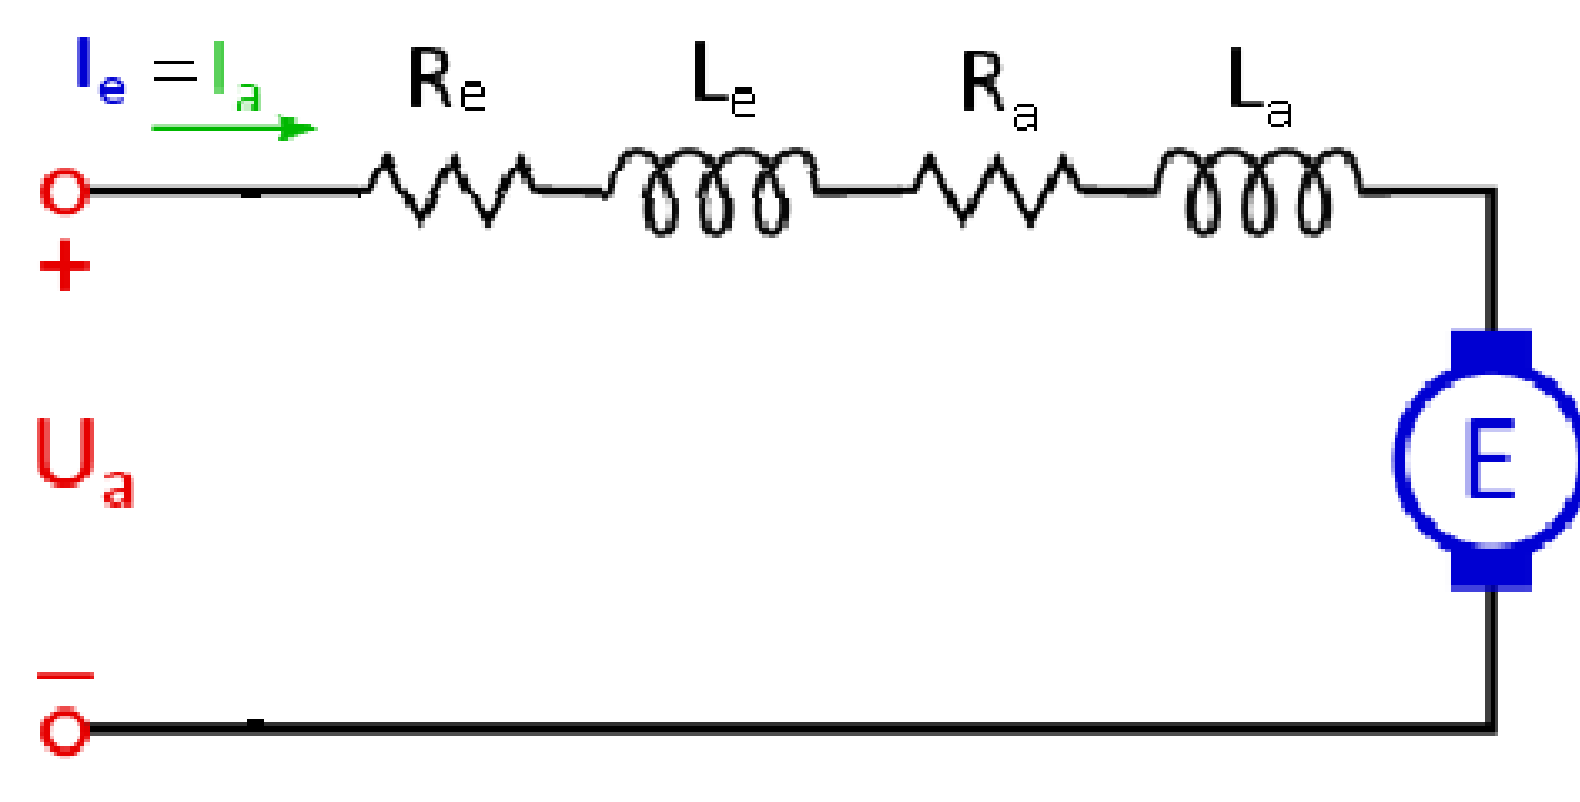
\includegraphics[width=0.6\textwidth]{assets/seriebekrachtiging.png}
     \caption{Serie bekrachtiging van een DC-machine}
     \label{fig:seriebekrachtiging.png}
    \end{figure}
\end{itemize}

Andere types motoren zijn:

\begin{itemize}
 \item \textbf{PMDC (Permanent Magnet DC)}:
 Deze zien we later nog in de cursus, dit is een DC-machine met permanente magneten in de
 rotor, dit is dus een synchrone machine.
 Deze heeft geen bekrachtiging nodig want de magneten zorgen voor het veld.
 \item \textbf{Compound}:
 Dit combineert de eigenschappen van zowel shunt- als serie-excitatie, waardoor het koppel
 en de snelheid beter gereguleerd kunnen worden.
 Het heeft zowel een parallelle als een seriële wikkeling.
 Deze motor komt weinig voor in de praktijk.
 \item \textbf{Borstelloze DC}:
 Zelfde T-n karakteristiek als een PMDC, maar de constructie lijkt op die van de synchrone
 machine.
\end{itemize}

\subsection{Karakteristieken}

\subsubsection{T-n karakteristiek}

\begin{warningbox}[Sommige delen hier zijn niet te vinden op de slides maar komen van
lesnotities + AI]
  Na de volgende berekening voor T, is het deel van de grafieken vooral door AI gecooked
  op basis van mijn lesnotities, want dat deel staat niet in de slides ma kwam wel in de
  les aan bod dus ik waarschuw dat het misschien niet zo vlot leest als de rest en
  mogelijks fouten in kunnen staan, de grafieken kloppen wel normaal al zowieso wat denkik
  ook het belangrijkste is.
  Die getallen bij die grafieken, zoals je zult zien, zijn random en hebben geen
  betekenis.
\end{warningbox}

Met de eerder opgestelde vergelijkingen kunnen we de T-n karakteristiek van de DC-machine
bepalen.
We weten dat:
\begin{align*}
    T = C \cdot \varphi \cdot i_a
\end{align*}
En dat:
\begin{align*}
    U_a = E + R_a \cdot i_a
\end{align*}
Invullen voor $i_a$ geeft:
\begin{align*}
    T = C \cdot \varphi \cdot \frac{U_a - E}{R_a}
\end{align*}
En invullen voor E geeft:
\begin{align*}
    T = \frac{C \cdot \varphi \cdot U_a}{R_a} - \frac{C^2 \cdot \varphi^2 \cdot \omega}{R_a}
\end{align*}
Hierbij zijn $E$, $i_a$ en $\omega$ variabelen die kunnen veranderen en $R_a$ een
parameter (constant).

{\color{red}Vanaf hier tot 'magnetisatiecurve' is het AI slop.}

\subsubsection{Aparte en shunt excitatie}
Bij aparte en shunt excitatie is het veld onafhankelijk van $i_a$, dus $\varphi \approx$
constant.
Uit $T = C\varphi i_a$, $U_a = E + R_a i_a$ en $E = C\varphi\omega$ volgt de
\textbf{lineaire} $T$-$\omega$ relatie:
\begin{align*}
    T = \frac{C \varphi U_a}{R_a} - \frac{C^2 \varphi^2}{R_a} \cdot \omega
\end{align*}

\begin{figure}[H]
\centering
\begin{tikzpicture}
\begin{axis}[xlabel={$n$}, ylabel={$T$}, xmin=0, xmax=10, ymin=0, ymax=11, axis lines=left, thick, domain=0:8, samples=50]
\addplot[blue] {10 - 1.25*x};
\end{axis}
\end{tikzpicture}
\caption{Kwalitatieve T-n karakteristiek bij aparte/shunt excitatie}
\end{figure}

\textbf{Snijpunten:} bij stilstand ($\omega=0$) is $E=0$, dus $i_{a,aanloop}=U_a/R_a$
(groot, want $R_a$ klein $\to$ aanloopweerstand nodig) en
$T_{aanloop} = C\varphi U_a/R_a$.
Bij onbelast ($T=0$) krijg je het nullasttoerental $\omega_0 = U_a/(C\varphi)$.

\subsubsection{Invloed van $U_a$ en $\varphi$ op de karakteristiek}
\textbf{$U_a$ aanpassen (aparte excitatie):} de helling $-C^2\varphi^2/R_a$ hangt niet af
van $U_a$, dus je krijgt \textbf{parallelle rechten}:
hogere $U_a$ $\to$ hoger $T_{aanloop}$ én hoger $\omega_0$, beide evenredig met $U_a$.
Elke rechte heeft dus zijn eigen nulpunt (snelheid waar $T=0$) -- dit gebruikt men om de
snelheid te regelen onder het nominale toerental.

\begin{figure}[H]
\centering
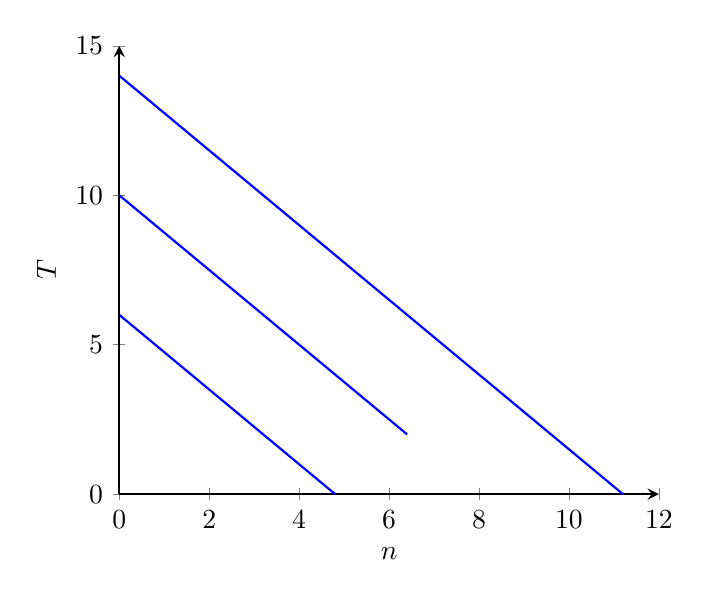
\begin{tikzpicture}
\begin{axis}[xlabel={$n$}, ylabel={$T$}, xmin=0, xmax=12, ymin=0, ymax=15, axis lines=left, thick]
\addplot[blue, domain=0:6.4, samples=50] {10 - 1.25*x};
\addplot[blue, domain=0:11.2, samples=50] {14 - 1.25*x};
\addplot[blue, domain=0:4.8, samples=50] {6 - 1.25*x};
\end{axis}
\end{tikzpicture}
\caption{Aanpassen van $U_a$ bij constante $\varphi$: parallelle rechten}
\end{figure}

\textbf{Let op bij shunt:} het veld hangt hier aan dezelfde voeding als het anker, dus als
je $U_a$ aanpast verandert $i_e$ (en dus $\varphi$) mee -- de rechten zijn dan
\textbf{niet} zuiver parallel.

\textbf{Veldverzwakking ($\varphi$ aanpassen bij constante $U_a$):} kleinere $\varphi$
geeft een \textbf{kleinere helling} (want $\varphi^2$ zit in de helling) $\to$ hoger
$\omega_0$ maar lager $T_{aanloop}$.
Dit gebruikt men om \textbf{boven} het nominale toerental te draaien, ten koste van
koppel.

\begin{figure}[H]
\centering
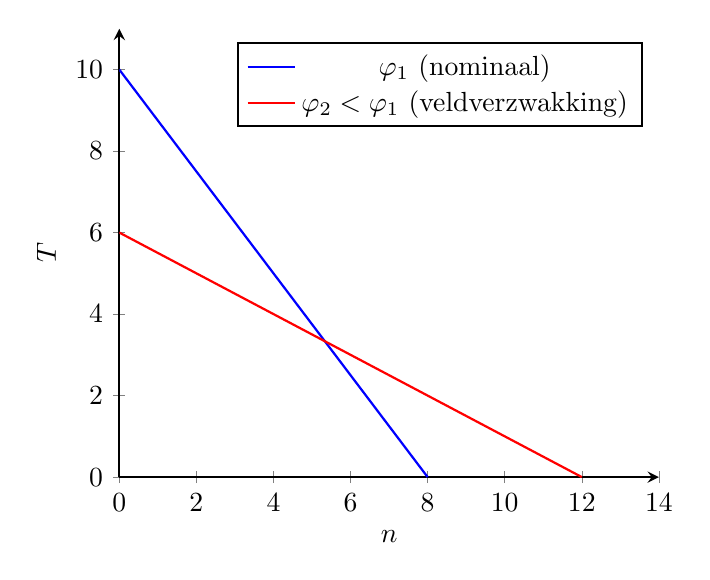
\begin{tikzpicture}
\begin{axis}[xlabel={$n$}, ylabel={$T$}, xmin=0, xmax=14, ymin=0, ymax=11, axis lines=left, thick, legend pos=north east]
\addplot[blue, domain=0:8, samples=50] {10 - 1.25*x};
\addlegendentry{$\varphi_1$ (nominaal)}
\addplot[red, domain=0:12, samples=50] {6 - 0.5*x};
\addlegendentry{$\varphi_2 < \varphi_1$ (veldverzwakking)}
\end{axis}
\end{tikzpicture}
\caption{Veldverzwakking: kleinere $\varphi$ geeft vlakkere rechte}
\end{figure}

\subsubsection{Serie excitatie}
Hier is $i_e = i_a$, hieruit volgt voor het koppel:
\begin{align*}
    T = G \cdot (\frac{U_a - E}{R_a})^2
\end{align*}
Dit is een \textbf{hyperboolachtige} curve, geen rechte.

\begin{figure}[H]
\centering
\begin{tikzpicture}
\begin{axis}[xlabel={$n$}, ylabel={$T$}, xmin=0, xmax=10, ymin=0, ymax=11, axis lines=left, thick, domain=0:10, samples=50]
\addplot[red] {10/((1+0.5*x)^2)};
\end{axis}
\end{tikzpicture}
\caption{Kwalitatieve T-n karakteristiek bij serie excitatie}
\end{figure}

\textbf{Belangrijk:} er is \textbf{geen} eindig nulpunt -- $\omega \to \infty$ als
$T \to 0$.
Een seriemotor mag dus \textbf{nooit onbelast draaien} (loopt op hol).

\subsubsection{Vergelijking}

\begin{figure}[H]
\centering
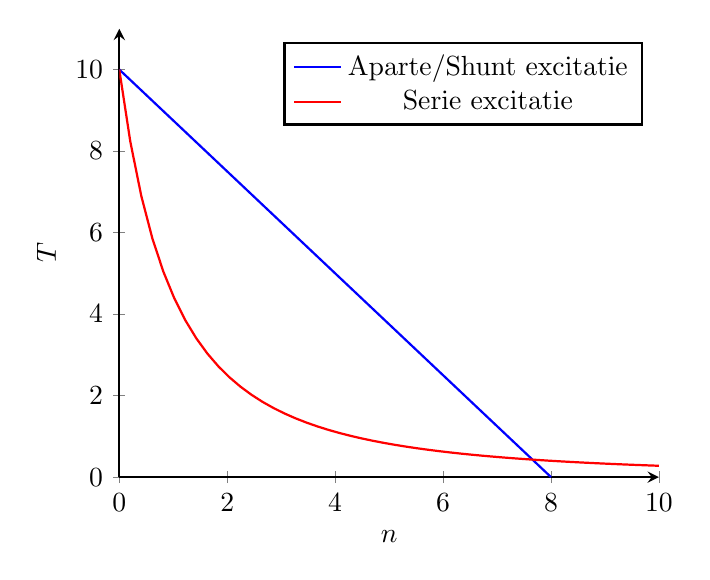
\begin{tikzpicture}
\begin{axis}[xlabel={$n$}, ylabel={$T$}, xmin=0, xmax=10, ymin=0, ymax=11, axis lines=left, thick, legend pos=north east]
\addplot[blue, domain=0:8, samples=50] {10 - 1.25*x};
\addlegendentry{Aparte/Shunt excitatie}
\addplot[red, domain=0:10, samples=50] {10/((1+0.5*x)^2)};
\addlegendentry{Serie excitatie}
\end{axis}
\end{tikzpicture}
\caption{Vergelijking van de T-n karakteristieken}
\end{figure}

\subsubsection{Constante ankerstroom}
Bij constante $i_a$ (en constante $\varphi$) is ook $T = C\varphi i_a$ constant,
onafhankelijk van $n$.
Omdat $E = C\varphi n$ een rechte door de oorsprong is, en $U_a = E + R_a i_a$ daar een
parallelle rechte van is, blijft de horizontale afstand tussen $U_a$ en $E$ overal gelijk
aan $R_a i_a$.

\begin{figure}[H]
\centering
\begin{tikzpicture}
    % Assen
    \draw[->] (0,0) -- (8,0) node[right] {$n$};
    \draw[->] (0,0) -- (0,7) node[above] {$T$};
    % Rode Ua-lijn: dalend, kruist n-as bij n_s
    \draw[red, thick] (0.3,6.5) -- (5,0);
    \node[red] at (0.6,7) {$U_a$ cte};
    % Blauwe E-lijn: verticaal, exact bij n_s
    \draw[blue, thick] (5,0) -- (5,6.5);
    \node[blue] at (5.4,7) {$E$ cte};
    \draw[dashed] (5,0) -- (5,-0.15);
    \node at (5,-0.4) {$n_s$};
    % Groene Ia-lijn: lager, los van Ua/E
    \draw[green!60!black, thick] (0,3) -- (7,3);
    \node[green!60!black] at (7.6,3) {$i_a$ cte};
    % Ra Ia pijl: HORIZONTAAL tussen rood en blauw, bovenaan
    \draw[<->, thick] (0.3,6.5) -- (5,6.5);
    \node at (2.65,6.8) {$R_a i_a$};
\end{tikzpicture}
\caption{Constante ankerstroom:
horizontale afstand tussen $U_a$ en $E$ = $R_a i_a$; ze vallen samen bij $T=0$ (op $n_s$)}
\end{figure}

\subsection{Magnetisatiecurve}
Nog iets belangrijks om rekening mee te houden is magnetisatie:
de flux $\varphi$ stijgt niet altijd lineair met de veldstroom $i_e$.
Bij lage veldstromen is dit wel het geval, maar naarmate de veldstroom stijgt, treedt
verzadiging op in het ijzer van de statorpolen.
Hierdoor neemt $\varphi$ minder snel toe met $i_e$, wat op zijn beurt de T-n
karakteristiek beïnvloedt.
De veldwikkeling heeft dus eigenlijk een nominale stroom:
voorbij die grens levert een hogere $i_e$ vooral opwarming in de spoelen op, want de
veldsterkte $H$ blijft dan wel toenemen, maar $B$ (en dus $\varphi$) niet meer.
De volgende grafiek toont deze magnetisatiecurve voor drie snelheidsgevallen
($N_3 > N_2 > N_1$), waarbij de veldstroom uitgezet is tegen de nullast-tegen-EMK (waar
het koppel 0 is):

\begin{figure}[H]
  \centering
  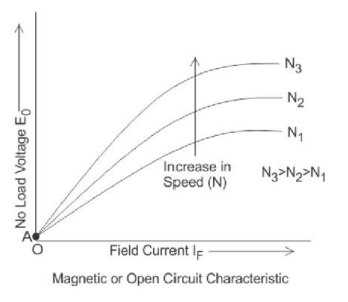
\includegraphics[width=0.5\textwidth]{assets/magnetisatiecurve.png}
  \caption{Magnetisatiecurve}
  \label{fig:magnetisatiecurve.png}
 \end{figure}

\newpage

\section{DC-motor problemen}
In het algemeen zijn er 3 problemen die kunnen optreden bij een DC-machine, deze zullen we
nu bespreken.

\subsection{Open veld circuit}
Dit zegt eigenlijk dat het heel gevaarlijk is om het veld van de DC-machine 'open te
zetten' (\textbf{onderbreken} eigenlijk).
Ik herhaal hier nog even de 3 vergelijkingen van hierboven:
\begin{align*}
    U_a &= E + R_a i_a \\
    E &= C \cdot \varphi \cdot \omega \\
    T &= C \cdot \varphi \cdot i_a
\end{align*}
Stel dus dat we het circuit van dat veld onderbreken, dus $i_e$ wordt heel klein, waardoor
het veld $\varphi$ ook heel klein wordt.
In de praktijk daalt $\varphi$ echter nooit helemaal tot nul:
door hysteresis in het ijzer blijft er een kleine \textbf{remanente flux} $\varphi_{rest}$
over, en die blijft hierna cruciaal.
Op het moment dat het veld wegvalt, wordt het koppel $T$ eerst heel klein, maar op dat
moment is de snelheid $\omega$ van de rotor nog steeds dezelfde en groot; ons tegen-emk
wordt wel kleiner doordat het veld kleiner wordt.
De klemspanning $U_a$ is constant, dus de volledige spanning gaat over dat $R_a \cdot i_a$
gedeelte staan, waardoor de stroom $i_a$ heel snel groot wordt en dus $R_a$ kan
doorbranden (\textit{anker opbranden}).
En omdat $i_a$ zo snel zo groot wordt, zorgt zelfs die kleine restflux $\varphi_{rest}$
voor een aanzienlijk koppel ($T=C\varphi_{rest} i_a$), waardoor de snelheid $\omega$ ook
heel groot gaat worden -- de snelheid gaat dus eigenlijk naar oneindig.
Dit is dus een gevaarlijke situatie, en daarom mag je het veld van een DC-machine nooit
open zetten.

\subsection{Commutator arcing (borstelvuur/vonken)}
We weten nu al dat de commutator uit veel aparte stukken bestaat, en dat de
koolstofborstels daar tegenaan drukken.
Terwijl de rotor draait, moet elke spoel op een bepaald moment van polariteit wisselen:
de borstel raakt dan heel even twee naburige commutatorlamellen tegelijk en sluit die
spoel kort, waarbij de stroom moet omkeren van $+i$ naar $-i$.
Omdat elke spoel een zelfinductie $L$ heeft, verzet ze zich tegen die snelle
stroomverandering via:
\begin{align*}
    u_L = L \cdot \frac{di}{dt}
\end{align*}
Omdat de omkering in een heel korte commutatieperiode moet gebeuren, is $di/dt$ groot, en
dus ook $u_L$.
Net op het moment dat het koperoppervlak van de lamel onder de borstel verdwijnt, wil de
stroom door die inductie nog blijven vloeien -- ze springt dan over het luchtspleetje
tussen borstel en lamel, ioniseert de lucht, en er ontstaat een vonk.
Die vonken vreten zowel de koolstofborstel als de lamellen weg, en bij hevige/chronische
vonkvorming kan dit escaleren tot \textbf{borstelvuur} (ringvuur):
een doorlopende boog over meerdere lamellen die de machine zwaar kan beschadigen.

Om dit te beperken gebruikt men \textbf{commutatiepolen} (hulppolen die $u_L$
compenseren), plaatst men de borstels op het \textbf{neutrale vlak}, en gebruikt men
\textbf{koolstof} als borstelmateriaal voor een geleidelijkere weerstandscommutatie.

Dit is dus wel iets dat voorkomt bij snelle snelheden, de snelheid beperken kan dus ook
dit effect verminderen.

\newpage

\subsection{Ankerreactie}
Een ander probleem dat kan optreden is de ankerreactie, dit is eigelijk \textbf{het effect
van het veld van de rotor op het veld van de stator}, het vervormt het veld van de stator
dus.
Dit is wat we eerder zagen, de wet van Ampère zegt dat een stroomvoerende geleider een
magnetisch veld opwekt, en de rotor is dus een stroomvoerende geleider.
Dit zorgt voor een fluxverlies, en dat het 'neutrale vlak' gaat draaien, dit zien we in de
volgende figuur:

\begin{figure}[H]
  \centering
  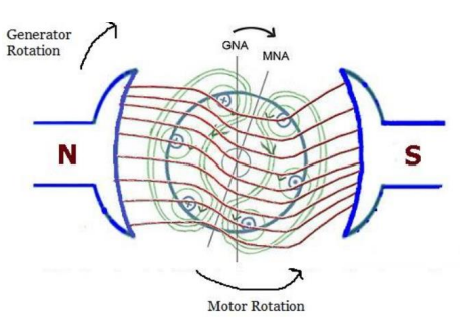
\includegraphics[width=0.5\textwidth]{assets/ankerreactie.png}
  \caption{Ankerreactie}
  \label{fig:ankerreactie.png}
 \end{figure}

Het 'neutrale vlak' (aangeduid met GNA) is het vlak waar de stroom door de rotor loodrecht
staat op het veld van de stator, en dus geen tegen-emk induceert.
Door de ankerreactie wordt dit vlak verschoven (aangeduid met MNA (modified)), waardoor de
commutatie niet meer optimaal is en er vonkvorming kan optreden.
Dit effect kan worden verminderd door het gebruik van commutatiepolen en door de juiste
plaatsing van de koolstofborstels (schuin dus, hoeveel hangt af van de stroom).
Er zijn dus trucjes om dit op te lossen maar dat moeten we niet kennen.

\newpage

\section{DC-motor oefeningen}

\begin{oefenblok}[Oefening 1 (Op slides)]
\textbf{Opgave:}
\newline
A shunt-connected 75kW, 250V DC motor has an armature resistance of 45mohm and a field
resistance of 185ohm.
When operated at 250V its no-load speed is 1850rpm.
The motor is operating under load at a terminal voltage of 250V and a terminal current of
290A.
\begin{itemize}
  \item a) Calculate the motor speed, load power, load torque in this operation point.
  \item b) Assuming the load torque remains constant as a function of speed, calculate the
  motor speed if the terminal voltage is reduced to 200V.
\end{itemize}
\textbf{Oplossing:}
\newline
We schrijven eerst eens rap onze gegevens op: 
\begin{itemize}
 \item $P = 75 kW$
 \item $U_a = 250 V$
 \item $R_a = 45 m\Omega$
 \item $R_{veld} = 185 \Omega$
 \item $n_{no,load} = 1850 rpm$
 \item $I = 290 A$
\end{itemize}
Teken altijd een schema van het circuit van de motor!
Hier is het shunt bekrachtigd, dus de opstelling, met al gegevens ingevuld ziet er zo uit:
\begin{figure}[H]
  \centering
  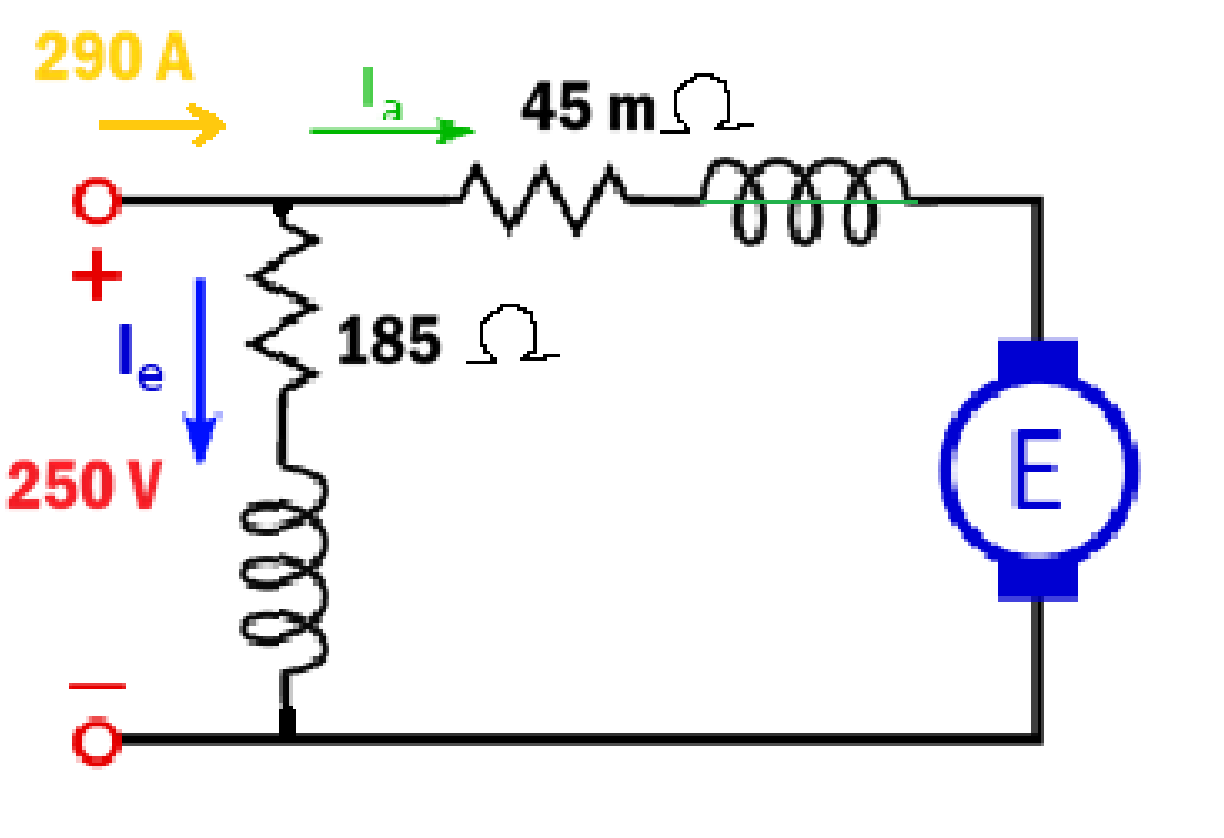
\includegraphics[width=0.5\textwidth]{assets/schemaoef1dc.png}
  \caption{Schema van de shunt-connected DC-motor Oefening 1}
  \label{fig:schemaoef1dc.png}
 \end{figure}
De spoel van rotor ($L_a$) is daar doorgetrokken met een groene lijn, we negeren deze want
de spanningsval hierover is zo goed als 0.

De snelheid van de motor kunnen we berekenen met de eerder gezien formule van het
tegen-emk:
\begin{align*}
    E = C \cdot \varphi \cdot \omega
\end{align*}
We hebben $C \cdot \varphi$ niet, maar we kunnen dit wel berekenen met de gegevens van de
no-load situatie, want hier is $E_0 = U_a - R_a \cdot I_a$ maar bij no-load is $I_a = 0$:
\begin{align*}
    C \cdot \varphi = \frac{E_0}{\omega} = \frac{U_a}{2 \pi n_{no,load}/60} = \frac{250}{2 \pi \cdot 1850/60} = 1.29 Vs
\end{align*}
We kunnen ook de veldstroom berekenen, want met deze stroom vinden we de ankerstroom:
\begin{align*}
    I_{veld} = \frac{U_a}{R_{veld}} = \frac{250}{185} = 1.35 A
\end{align*}
We kunnen nu de ankerstroom berekenen:
\begin{align*}
    I_a = I - I_{veld} = 290 - 1.35 = 288.65 A
\end{align*}
En met dit vinden we de tegen-emk van de motor:
\begin{align*}
    E = U_a - R_a \cdot I_a = 250 - 0.045 \cdot 288.65 = 237.01 V
\end{align*}
Dit invullen in de formule van het tegen-emk geeft ons de snelheid van de motor:
\begin{align*}
    n = \frac{E}{C \cdot \varphi} \cdot \frac{60}{2 \pi} = \frac{237.01}{1.29} \cdot \frac{60}{2 \pi} = 1753.5 rpm
\end{align*}
Het vermogen van de motor kunnen we berekenen met de formule:
\begin{align*}
    P_{last} = T \cdot \omega = T \cdot \frac{2 \pi n}{60}
\end{align*}
We hebben $T$ niet, maar we kunnen dit wel berekenen met de formule van het koppel:
\begin{align*}
    T = C \cdot \varphi \cdot I_a = 1.29 \cdot 288.65 = 372.2 Nm
\end{align*}
Invullen in de formule van het vermogen geeft ons:
\begin{align*}
    P_{last} = 372.2 \cdot \frac{2 \pi \cdot 1753.5}{60} = 68000 W = 68 kW
\end{align*}
\textbf{Deel b van de oefening:}
\newline
Nu daalt de klemspanning naar 200V, maar het koppel blijft constant, dus die
$T = 372.2 Nm$ blijft behouden.
Doordat de spanning daalt, zal de veldstroom dalen naar:
\begin{align*}
    I_{veld} = \frac{U_a}{R_{veld}} = \frac{200}{185} = 1.08 A
\end{align*}
De totale stroom zal ook veranderen, maar nu dat we weten dat het koppel constant blijft,
kunnen we de ankerstroom berekenen.
Dit doen we met:
\begin{align*}
    T = I_{a,2} \cdot C \cdot \varphi_2
\end{align*}
De factor $C \cdot \varphi_2$ kunnen we berekenen terug met de nullast situatie maar nu
met een klemspanning van 200V:
\begin{align*}
    C \cdot \varphi_2 = \frac{E_0}{\omega} = \frac{U_a}{2 \pi n_{no,load}/60} = \frac{200}{2 \pi \cdot 1850/60} = 1.03 Vs
\end{align*}
Invullen in de formule van het koppel geeft ons:
\begin{align*}
    I_{a,2} = \frac{T}{C \cdot \varphi_2} = \frac{372.2}{1.03} = 361.5
\end{align*}
We kunnen nu de tegen-emk berekenen:
\begin{align*}
    E_2 = U_a - R_a \cdot I_{a,2} = 200 - 0.045 \cdot 361.5 = 183.7 V
\end{align*}
En met dit vinden we de snelheid van de motor:
\begin{align*}
    n_2 = \frac{E_2}{C \cdot \varphi_2} \cdot \frac{60}{2 \pi} = \frac{183.7}{1.03} \cdot \frac{60}{2 \pi} = 1703.5 rpm
\end{align*}
\end{oefenblok}

Volgende oefening staat niet in de slides, maar wel op toledo.
Ik raad zeker aan deze te maken aangezien het grote deel van het examen op oefeningen telt
terwijl er geen oefensessies van dit vak zijn.

\begin{oefenblok}[Oefening 2 (Op Toledo)]
\textbf{Opgave:}
\newline
A four-pole, 25kW , 250V separately excited DC motor is mechanically coupled to a
threephase four-pole, 25kW, 460V, cylindrical pole synchronous generator.
The DC motor is connected to a constant 250V DC supply and the ac generator is connected
to a 460V fixed voltage, fixed frequency, threephase grid.
The synchronous reactance of the synchroous generator is 6.6 $\Omega$.
The armature resistance of the DC motor is 22 $m\Omega$.
All unspecified losses are to be neglected.
\begin{itemize}
 \item 1) If the two machines act as a motor-generator set receiving power from the DC
 source and delivering power to the ac grid, what is the internal phase voltage ESM of the
 ac machine when it delivers 25kW at unity power factor?
 What is the internal voltage (back-emf) of the DC motor?
 \item 2) Leaving the field current of the ac machine at the value corresponding to the
 condition of part (a), what adjustment can be made to reduce the power transfer between
 the two machines to zero?
 Under this condition of zero power transfer, what is the armature current of the DC
 machine?
 What is the armature current of the ac machine?
 \item 3) Leaving the field current of the ac machine as in parts (a) and (b), what
 adjustment can be made to cause the transfer of 25kW from tha ac source to the DC source?
 Under these conditions, what are the armature current and internal voltage of the DC
 machine?
 What will be the magnitude and phase of the current in the ac machine?
\end{itemize}
\textbf{Oplossing:}
\dots ({\color{red}Nog niet aan begonnen})
\end{oefenblok}

\newpage
